\subsection{Módulo de Campañas y Comunicación Masiva}\label{subsec:campanas}

El Módulo de Campañas fue diseñado para dotar a los operadores de la plataforma de una herramienta centralizada y eficiente para la captación, fidelización y comunicación directa con clientes potenciales. El módulo orquesta la gestión de información de contacto y facilita el envío proactivo de mensajes a través de múltiples canales. Su implementación abarcó tanto el diseño de la interfaz de administración como la construcción de la arquitectura \textit{backend} orientada al procesamiento de altos volúmenes de envíos.

\subsubsection{Interfaz de Administración y Experiencia de Usuario}

Para el portal administrativo, se implementó un conjunto de vistas interactivas destinadas al control completo sobre las operaciones de comunicación. La interfaz central del módulo ofrece una visualización tabular y estructurada donde los administradores pueden ejecutar el ciclo completo de gestión —creación, lectura, actualización y eliminación— sobre las campañas registradas. La \autoref{fig:campaigns-table} ilustra esta vista principal, donde cada fila de la tabla corresponde a una campaña con sus indicadores de estado, canal de envío y métricas de alcance, proporcionando una visión operativa integral al administrador.

\newcommand\campaignsTableCaption{Vista principal del módulo de campañas con listado tabular y operaciones CRUD sobre los registros. \hspace{1em}}
\begin{figure}[H]
  \centering
  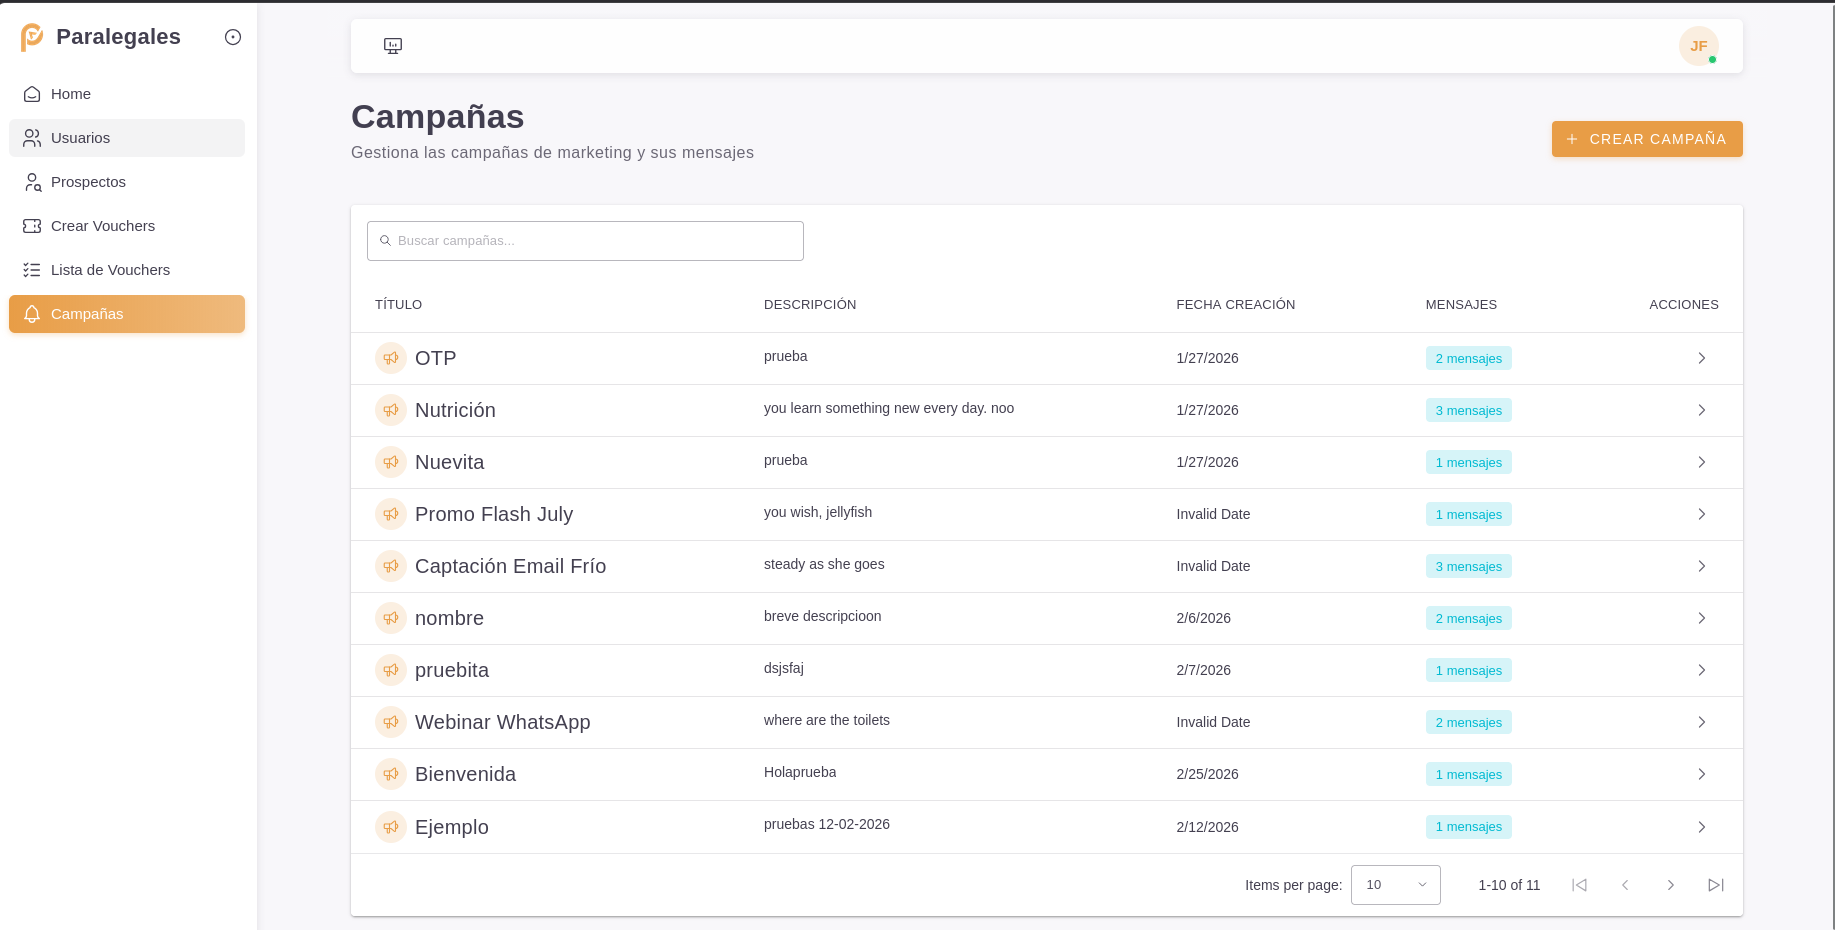
\includegraphics[width=1\textwidth]{img/figures/fig29-campaings-table.png}
  \caption[\campaignsTableCaption]{\campaignsTableCaption Fuente: Elaboración propia.}
  \label{fig:campaigns-table}
\end{figure}

Con el objetivo de maximizar la productividad y minimizar la fricción durante la navegación, se desarrolló un sistema de paneles laterales contextuales (\textit{sidebars}) que permite configurar los parámetros de envío, redactar mensajes y previsualizar el contenido sin abandonar la vista principal.

Adicionalmente, se diseñaron cuadros de diálogo especializados para ejecutar operaciones sobre campañas individuales. La \autoref{fig:editar-campana} presenta el formulario de edición de una campaña existente, que permite al administrador modificar sus atributos principales —nombre, descripción, canal y estado— desde un diálogo modal que preserva el contexto de la lista subyacente.

\newcommand\editarCampanaCaption{Diálogo de edición de una campaña existente con formulario de actualización de atributos principales. \hspace{1em}}
\begin{figure}[H]
  \centering
  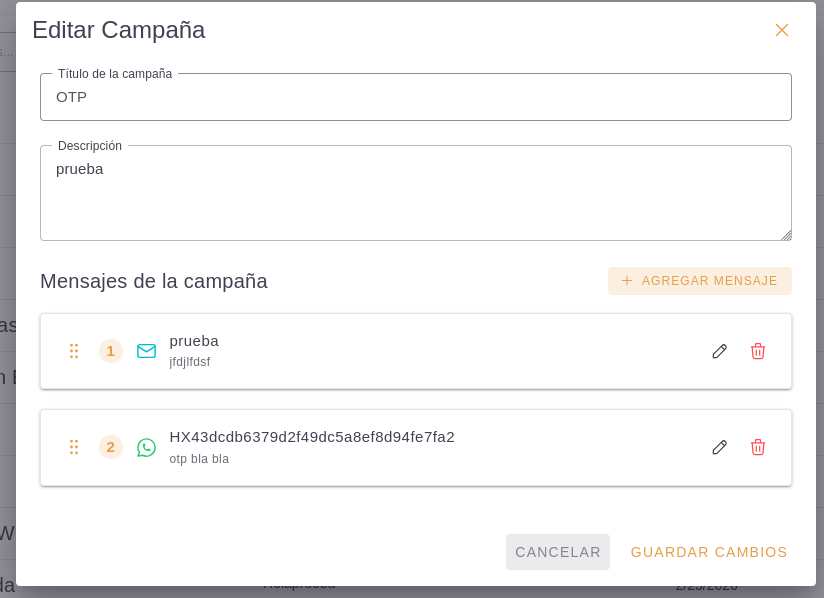
\includegraphics[width=0.85\textwidth]{img/figures/fig31-editar-campaing.png}
  \caption[\editarCampanaCaption]{\editarCampanaCaption Fuente: Elaboración propia.}
  \label{fig:editar-campana}
\end{figure}

Dentro de estos paneles, se incorporó una funcionalidad de plantillas dinámicas que permite insertar variables personalizadas —como el nombre del destinatario o detalles específicos de su caso—, las cuales son interpretadas y reemplazadas por el sistema en el momento del envío. La \autoref{fig:editar-mensaje} muestra el editor de contenido del mensaje, donde el administrador puede redactar el texto de la comunicación e insertar variables dinámicas mediante una interfaz asistida, con una previsualización del resultado final antes de ejecutar el envío masivo.

\newcommand\editarMensajeCaption{Editor de plantillas de mensaje con soporte para variables dinámicas personalizadas. \hspace{1em}}
\begin{figure}[H]
  \centering
  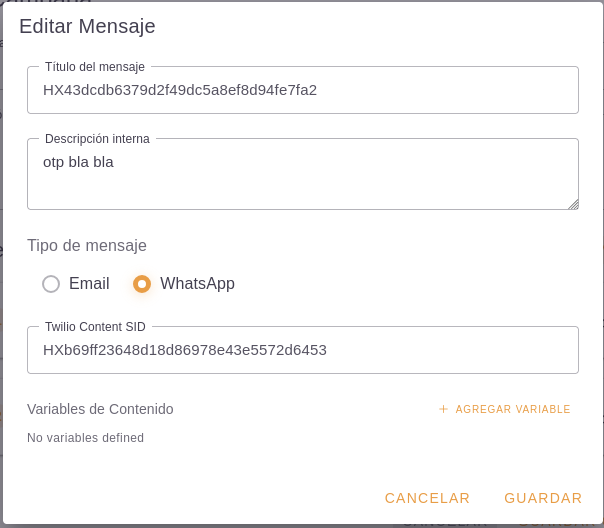
\includegraphics[width=0.85\textwidth]{img/figures/fig32-editar-msg.png}
  \caption[\editarMensajeCaption]{\editarMensajeCaption Fuente: Elaboración propia.}
  \label{fig:editar-mensaje}
\end{figure}

A nivel estructural en el \textit{frontend}, el módulo fue construido bajo un paradigma de componentes modulares y reutilizables, separando la presentación de la lógica de negocio. Se establecieron modelos estrictos de información para representar las entidades de campañas y clientes potenciales, complementados con un sistema de gestión de estado global que sincroniza reactivamente las interacciones del administrador con la base de datos documental en tiempo real, garantizando que cualquier modificación en los parámetros de una campaña se refleje de forma instantánea en todas las vistas de la plataforma.

\subsubsection{Procesamiento \textit{Backend} y Orquestación de Envíos Masivos}

El principal desafío técnico del módulo residía en la capacidad del sistema para procesar altos volúmenes de envíos sin degradar el rendimiento de la aplicación cliente ni incurrir en tiempos de espera prolongados (\textit{timeouts}). Para resolver esto, se diseñó e implementó una arquitectura \textit{backend} asíncrona basada en microservicios y funciones \textit{serverless}.

Cuando el administrador confirma un envío masivo desde el panel, el cliente transmite una solicitud estructurada hacia la nube. Esta petición es interceptada por una función bajo demanda que actúa como orquestadora: su responsabilidad principal no es enviar los mensajes de manera inmediata, sino validar la solicitud, desglosar el volumen total de destinatarios y depositar las instrucciones individuales de envío en el sistema de colas de mensajería SQS. Esta abstracción mediante colas desacopla por completo la experiencia del administrador de la latencia de red de los proveedores externos de mensajería. Posteriormente, otras funciones especializadas consumen estas colas, interpretan las variables dinámicas configuradas desde la interfaz y enrutan cada mensaje hacia el proveedor correspondiente —como servicios de correo electrónico o plataformas de mensajería instantánea—.

Para garantizar la fiabilidad técnica de la operación, se integraron capas de observabilidad y registro de eventos en cada punto del ciclo de vida del mensaje, permitiendo trazar el estado de una comunicación desde su origen en el panel de administración, su paso por el sistema de colas, hasta su entrega final. Esta arquitectura asíncrona constituye, de hecho, uno de los casos de uso más representativos del sistema de observabilidad transversal que se describe en el siguiente apartado.
